\documentclass{standalone}
\usepackage{tikz-network}
\begin{document}
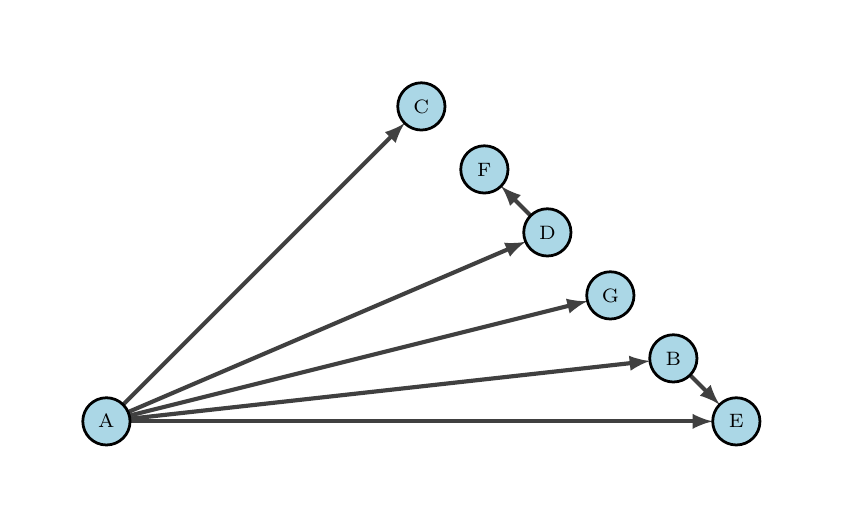
\begin{tikzpicture}
\clip (0,0) rectangle (10.0,6.0);
\Vertex[x=1.000,y=1.000,label=A]{A}
\Vertex[x=8.200,y=1.800,label=B]{B}
\Vertex[x=5.000,y=5.000,label=C]{C}
\Vertex[x=6.600,y=3.400,label=D]{D}
\Vertex[x=7.400,y=2.600,label=G]{G}
\Vertex[x=5.800,y=4.200,label=F]{F}
\Vertex[x=9.000,y=1.000,label=E]{E}
\Edge[,Direct](A)(B)
\Edge[,Direct](A)(C)
\Edge[,Direct](A)(D)
\Edge[,Direct](A)(G)
\Edge[,Direct](A)(E)
\Edge[,Direct](B)(E)
\Edge[,Direct](D)(F)
\end{tikzpicture}
\end{document}